\documentclass[border=6pt]{standalone}
\usepackage{tikz}
\usetikzlibrary{arrows.meta,positioning,fit,calc,backgrounds}
\definecolor{fg}{HTML}{3B3220}
\definecolor{fgbody}{HTML}{544736}
\definecolor{stroke}{HTML}{7A5A10}
\definecolor{surf}{HTML}{F4F5F8}
\definecolor{surfemph}{HTML}{E6E8EE}
\definecolor{surfact}{HTML}{FDE8E8}
\definecolor{bdim}{HTML}{CFC6B2}
\definecolor{bemph}{HTML}{7A5A10}
\definecolor{bact}{HTML}{8F1D1D}
\begin{document}
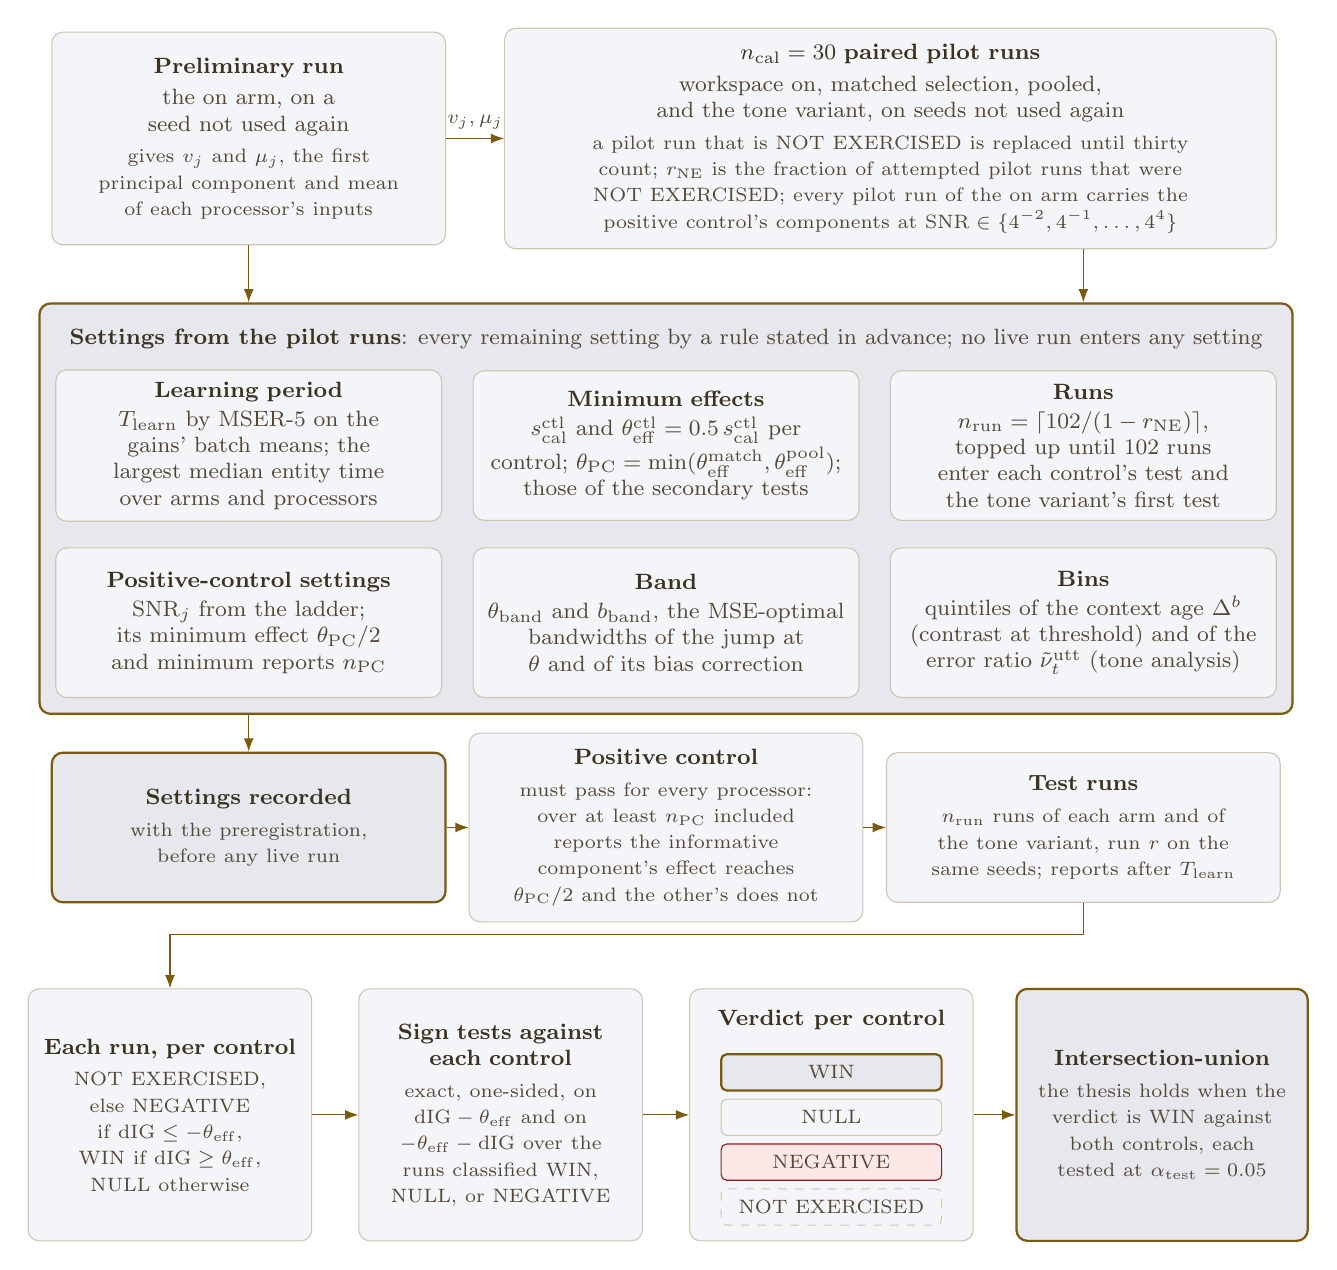
\begin{tikzpicture}[
  font=\small,>=Latex,
  every node/.append style={text=fgbody},
  every node/.append style={execute at begin node={\hyphenpenalty=10000\exhyphenpenalty=10000\thickmuskip=5mu\medmuskip=4mu}},
  mod/.style={draw=bdim, rounded corners, fill=surf, align=center, font=\footnotesize, inner sep=2mm},
  on/.style={draw=bemph, thick, rounded corners, fill=surfemph, align=center, font=\footnotesize, inner sep=2mm},
  cell/.style={draw=bdim, rounded corners, fill=surf, align=center, font=\footnotesize, text width=46mm, minimum height=19mm, inner sep=1.5mm},
  dec/.style={draw=bdim, rounded corners, fill=surf, align=center, font=\footnotesize, text width=33mm, minimum height=32mm, inner sep=1.5mm},
  chip/.style={draw=bdim, rounded corners=2pt, fill=surf, align=center, font=\scriptsize, minimum width=28mm, minimum height=4.6mm, inner sep=1pt},
  lbl/.style={font=\scriptsize, text=fgbody, align=center},
]
% 1. preliminary run and pilot runs
\node[mod, text width=46mm, minimum height=27mm] (pre) at (2.7,0)
  {\textcolor{fg}{\textbf{Preliminary run}}\\[2pt]the on arm, on a seed not used again\\[2pt]\scriptsize gives $v_j$ and $\mu_j$, the first principal component and mean of each processor's inputs};
\node[mod, text width=94mm, minimum height=27mm] (pil) at (10.85,0)
  {\textcolor{fg}{\textbf{$n_{\rm cal}=30$ paired pilot runs}}\\[2pt]workspace on, matched selection, pooled, and the tone variant, on seeds not used again\\[2pt]\scriptsize a pilot run that is NOT EXERCISED is replaced until thirty count; $r_{\rm NE}$ is the fraction of attempted pilot runs that were NOT EXERCISED; every pilot run of the on arm carries the positive control's components at $\mathrm{SNR}\in\{4^{-2},4^{-1},\dots,4^{4}\}$};
\draw[->, draw=stroke] (pre) -- node[lbl, above]{$v_j,\mu_j$} (pil);
% 2. settings from the pilot runs
\node[cell] (c1) at (2.7,-3.9)
  {\textcolor{fg}{\textbf{Learning period}}\\[1pt]$T_{\rm learn}$ by MSER-5 on the gains' batch means; the largest median entity time over arms and processors};
\node[cell] (c2) at (8.0,-3.9)
  {\textcolor{fg}{\textbf{Minimum effects}}\\[1pt]$s^{\rm ctl}_{\rm cal}$ and $\theta^{\rm ctl}_{\rm eff}=0.5\,s^{\rm ctl}_{\rm cal}$ per control; $\theta_{\rm PC}=\min(\theta^{\rm match}_{\rm eff},\theta^{\rm pool}_{\rm eff})$; those of the secondary tests};
\node[cell] (c3) at (13.3,-3.9)
  {\textcolor{fg}{\textbf{Runs}}\\[1pt]$n_{\rm run}=\lceil 102/(1-r_{\rm NE})\rceil$, topped up until 102 runs enter each control's test and the tone variant's first test};
\node[cell] (c4) at (2.7,-6.15)
  {\textcolor{fg}{\textbf{Positive-control settings}}\\[1pt]$\mathrm{SNR}_j$ from the ladder; its minimum effect $\theta_{\rm PC}/2$ and minimum reports $n_{\rm PC}$};
\node[cell] (c5) at (8.0,-6.15)
  {\textcolor{fg}{\textbf{Band}}\\[1pt]$\theta_{\rm band}$ and $b_{\rm band}$, the MSE-optimal bandwidths of the jump at $\theta$ and of its bias correction};
\node[cell] (c6) at (13.3,-6.15)
  {\textcolor{fg}{\textbf{Bins}}\\[1pt]quintiles of the context age $\Delta^b$ (contrast at threshold) and of the error ratio $\tilde\nu^{\rm utt}_t$ (tone analysis)};
\node[font=\footnotesize, anchor=south, align=center] (tooltitle) at ($(c2.north)+(0,1.5mm)$)
  {\textcolor{fg}{\textbf{Settings from the pilot runs}}: every remaining setting by a rule stated in advance; no live run enters any setting};
\begin{pgfonlayer}{background}
\node[draw=bemph, thick, rounded corners, fill=surfemph, fit=(tooltitle)(c1)(c3)(c4)(c6), inner sep=2mm] (tool) {};
\end{pgfonlayer}
\draw[->, draw=stroke] (pil.south -| c3) -- (tool.north -| c3);
\draw[->, draw=stroke] (pre.south) -- (tool.north -| pre);
% 3. settings record, positive control, test runs
\node[on, text width=46mm, minimum height=19mm] (rec) at (2.7,-8.75)
  {\textcolor{fg}{\textbf{Settings recorded}}\\[2pt]\scriptsize with the preregistration, before any live run};
\node[mod, text width=46mm, minimum height=19mm] (pc) at (8.0,-8.75)
  {\textcolor{fg}{\textbf{Positive control}}\\[2pt]\scriptsize must pass for every processor: over at least $n_{\rm PC}$ included reports the informative component's effect reaches $\theta_{\rm PC}/2$ and the other's does not};
\node[mod, text width=46mm, minimum height=19mm] (runs) at (13.3,-8.75)
  {\textcolor{fg}{\textbf{Test runs}}\\[2pt]\scriptsize $n_{\rm run}$ runs of each arm and of the tone variant, run $r$ on the same seeds; reports after $T_{\rm learn}$};
\draw[->, draw=stroke] (tool.south -| rec) -- (rec);
\draw[->, draw=stroke] (rec) -- (pc);
\draw[->, draw=stroke] (pc) -- (runs);
% 4. decision rule
\node[dec] (d1) at (1.7,-12.4)
  {\textcolor{fg}{\textbf{Each run, per control}}\\[2pt]\scriptsize NOT EXERCISED, else NEGATIVE if \mbox{$\mathrm{dIG}\le-\theta_{\rm eff}$}, WIN if \mbox{$\mathrm{dIG}\ge\theta_{\rm eff}$}, NULL otherwise};
\node[dec] (d2) at (5.9,-12.4)
  {\textcolor{fg}{\textbf{Sign tests against each control}}\\[2pt]\scriptsize exact, one-sided, on \mbox{$\mathrm{dIG}-\theta_{\rm eff}$} and on \mbox{$-\theta_{\rm eff}-\mathrm{dIG}$} over the runs classified WIN, NULL, or NEGATIVE};
\node[dec] (d3) at (10.1,-12.4) {};
\node[font=\footnotesize, align=center, anchor=north] (d3t) at ($(d3.north)+(0,-1.5mm)$) {\textcolor{fg}{\textbf{Verdict per control}}};
\node[chip, fill=surfemph, draw=bemph, thick] (vw) at ($(d3.center)+(0,5.4mm)$) {WIN};
\node[chip] (vn) at ($(d3.center)+(0,-0.3mm)$) {NULL};
\node[chip, fill=surfact, draw=bact] (vneg) at ($(d3.center)+(0,-6.0mm)$) {NEGATIVE};
\node[chip, dashed] (vne) at ($(d3.center)+(0,-11.7mm)$) {NOT EXERCISED};
\node[on, text width=33mm, minimum height=32mm] (d4) at (14.3,-12.4)
  {\textcolor{fg}{\textbf{Intersection-union}}\\[2pt]\scriptsize the thesis holds when the verdict is WIN against both controls, each tested at $\alpha_{\rm test}=0.05$};
\draw[->, draw=stroke] (runs.south) -- ++(0,-4mm) -| (d1.north);
\draw[->, draw=stroke] (d1) -- (d2);
\draw[->, draw=stroke] (d2) -- (d3);
\draw[->, draw=stroke] (d3) -- (d4);
\end{tikzpicture}
\end{document}
